\chapter{Evaluation} 

\label{Chapter5}

\lhead{Chapter 5. Evaluation} 
To evaluate the performance of our network stack, we run experiments on the Cloudlab network testbed. We utilize two c220g2 servers  configured with two Intel E5-2660 v3 10-core Haswell CPUs, 160 GB RAM, and a dual-port Intel X520 10Gb NIC. We disable hyperthreading and set the CPUs to a constant frequency of 2.6GHz to reduce the variance in benchmarking. 

\section{L2 Forward}
We use DPDK's L2Forward example and benchmark it against a similar implementation in Rust. We vary the packet size from 100-1500 in steps of 100 with a batch size of 32 for both the implementations and sent packets at a rate of 10Gb/s (the line rate of the NIC). Since the CPU can easy saturate a 10Gb/s line while running at 2.6GHz, we also compare the performance at a frequency of 1GHz. 

\begin{figure}[!htbp]
	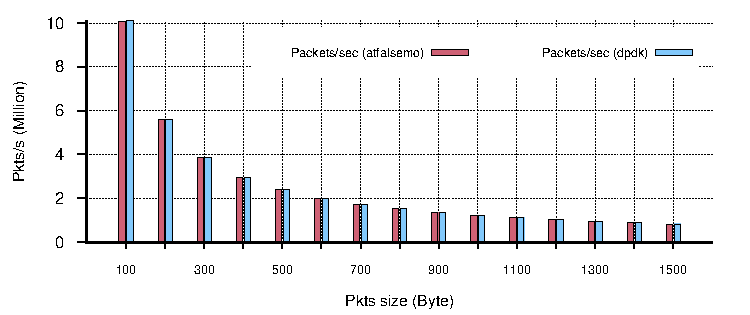
\includegraphics[width=1.0\columnwidth]{figures/l2fwd26.pdf}
\caption{L2Forward throughput measured at 2.6GHz}
	\label{fig:l2fwd26}
\end{figure}

\tirth{Add 1GHz benchmark for Ixy}

\section{Key-Value Store}
To study the overheads of our network stack on a realistic workload, we implement an in-memory key-value store backed by a hash-table based on the Fowler-Noll-Vo algorithm. Processing a packet consists of parsing the request, performing an insert/fetch operation in the hash table, filling the response buffer queuing the packet in the send batch. Transmitting a packet takes fewer cycles than receiving because calls to \lstinline{rx_batch} wait till the NIC is done writing packets into the DMA buffers while \lstinline{tx_batch} simply holds the DMA buffers in a private queue and the NIC can write to them asynchronously. The next time \lstinline{tx_batch} is called, the queue is cleaned and the buffers are returned as ``free buffers".

\tirth{Add key-value store table}
